\documentclass[12pt]{article}
\usepackage{tikz}
\usetikzlibrary{arrows,shapes}
\usepackage{helvet}

% \setpagesize{width}{height}   {margin}
\newcommand{\setpagesize}[2]{
  \setlength{\pdfpagewidth}{#1}
  \setlength{\pdfpageheight}{#2}
  %\addtolength{\pdfpageheight}{#3}
  %\addtolength{\pdfpagewidth}{#3}
  \setlength{\textheight}{\pdfpageheight}
  \setlength{\textwidth}{\pdfpagewidth}
  %\setlength\topmargin{-1in}
  \setlength{\voffset}{-1in}
  \setlength{\topmargin}{0in}
  \setlength{\headheight}{0in}
  \setlength{\headsep}{0in}
  \setlength{\footskip}{0in}
  \setlength{\hoffset}{-1in}
  %\setlength{\oddsidemargin}{-1in}
  %\setlength{\evensidemargin}{-1in}
  \setlength{\oddsidemargin}{0in}
  \setlength{\evensidemargin}{0in}
  \setlength{\marginparwidth}{0in}
  \setlength{\marginparpush}{0in}
  \setlength{\marginparsep}{0in}
  \setlength{\parindent}{0in}
  \setlength{\parskip}{0in}
}


%% see   getbb.sh  to find the bounding-box of the ink in a figure.

%% The sizes shown are from getbb.sh using 12pt font in figures.

%% pgf/tikz often believes that the bounding-box extends beyond the
%% extent of the ink, so forcing it to the ink size doesn't always
%% work (the figure overflows onto page 2)

% 169 x 65
\newcommand{\pointerlessfigwidth}{170pt}
\newcommand{\pointerlessfigheight}{76pt}

% 267 x 249
\newcommand{\permutefigwidth}{268pt}
\newcommand{\permutefigheight}{249pt}

% 251 x 162
\newcommand{\applypermfigwidth}{252pt}
\newcommand{\applypermfigheight}{162pt}

% 263 x 119
\newcommand{\ronlyfigwidth}{268pt}
\newcommand{\ronlyfigheight}{122pt}

% 233 x 93
\newcommand{\transposefigwidth}{234pt}
\newcommand{\transposefigheight}{93pt}

% 145 x 58
\newcommand{\bitpackfigwidth}{149pt}
\newcommand{\bitpackfigheight}{66pt}


\setpagesize{\transposefigwidth}{\transposefigheight}
\begin{document}%
\thispagestyle{empty}%
\begin{center}%
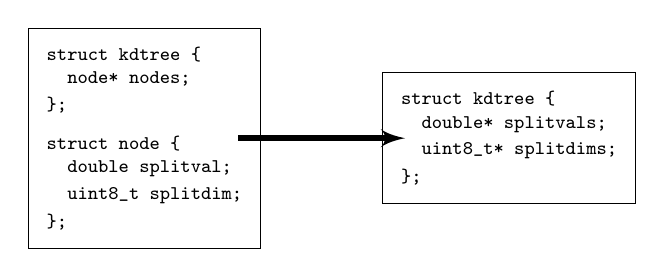
\begin{tikzpicture}[>=latex', font=\scriptsize]

  \tikzstyle{code}=[draw=black,
    execute at begin cell=\node\bgroup\tt,
    execute at end cell=\egroup;,
    anchor=west,
    row sep=-0.3em]

  \node [matrix, code] (before) at (0,0) {
\verb+struct kdtree {+\\
\verb+  node* nodes;+\\
\verb+};+\\
\rule{0pt}{1pt} \\
\verb+struct node {+\\
\verb+  double splitval;+\\
\verb+  uint8_t splitdim;+\\
\verb+};+\\
};


  \node [matrix, code] (after) at (4.5,0) {
\verb+struct kdtree {+\\
\verb+  double* splitvals;+\\
\verb+  uint8_t* splitdims;+\\
\verb+};+\\
};

\path [inner sep=0, minimum size=0]
(before.east)+(-0.3,0) node (n1) {} --
(after.west) +(0.3,0) node (n2) {};

\draw
[black, line width=2pt, ->]
(n1) to (n2);

\end{tikzpicture}%
\end{center}%
\end{document}
